\documentclass[10pt,a4paper]{article}

%%%%%%%%%%%%%%%%%%%%%%%%%%%
% MODIFY:

\newcommand{\authorA}{Ahmad Bin Qasim (03693345)}
\newcommand{\authorB}{Kaan Atukalp (03709123)}
\newcommand{\authorC}{Martin Meinel (03710370)}
\newcommand{\groupNumber}{H} % - YOUR GROUP NUMBER
\newcommand{\exerciseNumber}{5} % - THE NUMBER OF THE EXERCISE
\newcommand{\sourceCodeLink}{https://gitlab.lrz.de/ga53rog/praktikum-ml-crowd}

\newcommand{\workPerAuthor}{
\authorA&Task 1&33\%\\
      &Task 2&33\%\\
      &Task 3&33\%\\
      &Task 4&33\%\\
      & Task 5&33\%\\
      \hline
\authorB&Task 1&33\%\\
      &Task 2&33\%\\
      &Task 3&33\%\\
      &Task 4&33\%\\
      & Task 5&33\%\\
      \hline
\authorC&Task 1&33\%\\
      &Task 2&33\%\\
      &Task 3&33\%\\
      &Task 4&33\%\\
      & Task 5&33\%\\
}

%%%%%%%%%%%%%%%%%%%%%%%%%%%

%%
% imports for the exercise sheets
%

\usepackage[utf8]{inputenc}
\usepackage{amsmath}
\usepackage{amsfonts}
\usepackage{amssymb}

\usepackage[yyyymmdd]{datetime}
\renewcommand{\dateseparator}{--}

\usepackage[left=2cm,right=2cm,top=3cm,bottom=3cm]{geometry}

\usepackage{hyperref}

\usepackage{amsthm}
\newtheorem{lem}{Lemma}
\newtheorem{thm}{Theorem}
\newtheorem{cor}{Corollary}
\newtheorem{rem}{Remark}
\newtheorem{definition}{Definition}
\newtheorem{ter}{Terminology}

\usepackage{graphicx}

\newcommand{\M}{\mathcal{M}}
\newcommand{\N}{\mathcal{N}}
\newcommand{\K}{\mathcal{K}}
\newcommand{\SPDk}{\mathbb{P}^k}
\newcommand{\vol}{\text{vol}}

\newcommand{\Figref}[1]{Figure~\ref{#1}}
\newcommand{\figref}[1]{figure~\ref{#1}}
\newcommand{\Eqnref}[1]{Equation~(\eqref{#1})}
\newcommand{\eqnref}[1]{equation~(\eqref{#1})}

\usepackage{float}
\usepackage{tabularx}
\usepackage{subcaption}
\usepackage{mwe}

\usepackage{fancyhdr}
\pagestyle{fancy}

\usepackage{totcount}
\newtotcounter{taskCounter}
\newtotcounter{pointCounter}
\newenvironment{task}[1]{\noindent\stepcounter{taskCounter}\textbf{Report on task #1}\smallbreak\hrule\smallbreak}{\smallbreak\hrule\bigbreak}


\title{Report for exercise \exerciseNumber~from group~\groupNumber}

\makeatletter
\let\thetitle\@title
\let\theauthor\@author
\let\thedate\@date
\makeatother

\providecommand{\versiondate}{\today}

\lhead{Exercise sheet \exerciseNumber}
\chead{Master Praktikum: Modelling and Simulation of Crowds WS2019/20}
\rhead{TUM}
\lfoot{Report of Group \groupNumber}
\cfoot{\thepage}
\rfoot{Last compiled: \versiondate}
\renewcommand{\headrulewidth}{0.4pt}
\renewcommand{\footrulewidth}{0.4pt}

\newcommand{\frontpage}{
\begin{center}
\textbf{\thetitle}\\~\\
\end{center}
\begin{table}[H]
\begin{tabular}{ll}
Tasks addressed:&\total{taskCounter}\\
Authors:&\authorA\\
&\authorB\\
&\authorC\\
Last compiled:&\versiondate\\
Source code:&\sourceCodeLink
\end{tabular}
\end{table}
\vfill
The work on tasks was divided in the following way:
\begin{table}[H]
\begin{tabularx}{\textwidth}{X|p{2cm}|p{2cm}}
\workPerAuthor
\end{tabularx}
\end{table}
\newpage
}

\begin{document}

\frontpage

\begin{task}{1, Approximating functions}
Part 1: \bigbreak
For part 1 we loaded the linear data from the "linear\_function.txt" file and tried to approximate the function linearly. We used a linear regression model to minimize the least square error. For this problem there exists a closed form solution to compute the matrix A which contains the parameters to map the input to the output with a minimal least square error to the original function, we want to approximate. 
The least squares error problem is defined by following equation:
\begin{equation*}
\min_{\hat{f}}e(\hat{f}) = \min_{\hat{f}}||F-\hat{f}(X)||^2 = \min_{A}||F-XA^T||^2
\end{equation*}
Figure \ref{fig:task1_1} shows the original linear data in blue and its linear approximation in orange. It can be easily seen that all data points are laying on the linear straight which was computed with the closed form solution. The data is linear so the function can be approximated perfectly.
\begin{figure}[H]
\centering
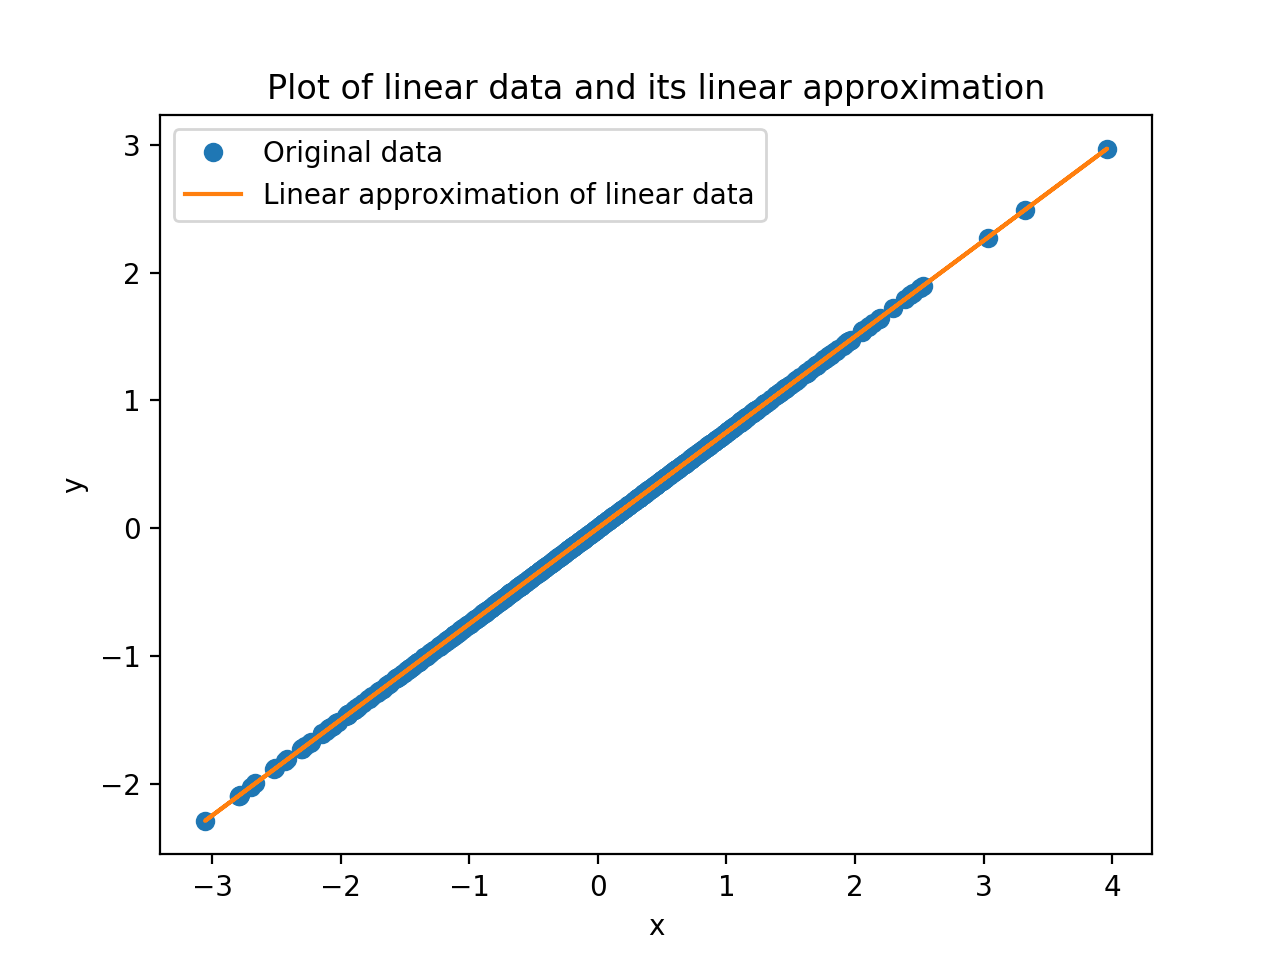
\includegraphics[width=0.7\textwidth]{../plots/task1_part1.png}
\caption{Plot of the linear data and its linear approximation}
\label{fig:task1_1}
\end{figure}
Part 2:
In the second part we use a nonlinear dataset from the "nonlinear\_function.txt" file and tried to approximate the function in a linear way again.
Figure \ref{fig:task1_2} shows then original data in blue again. The linear approximation of the function is  shown in orange. It can be easily seen that the linear approximation fits very bad. The reason for that is that the function is nonlinear and we try to approximate it linearly.
\begin{figure}[H]
\centering
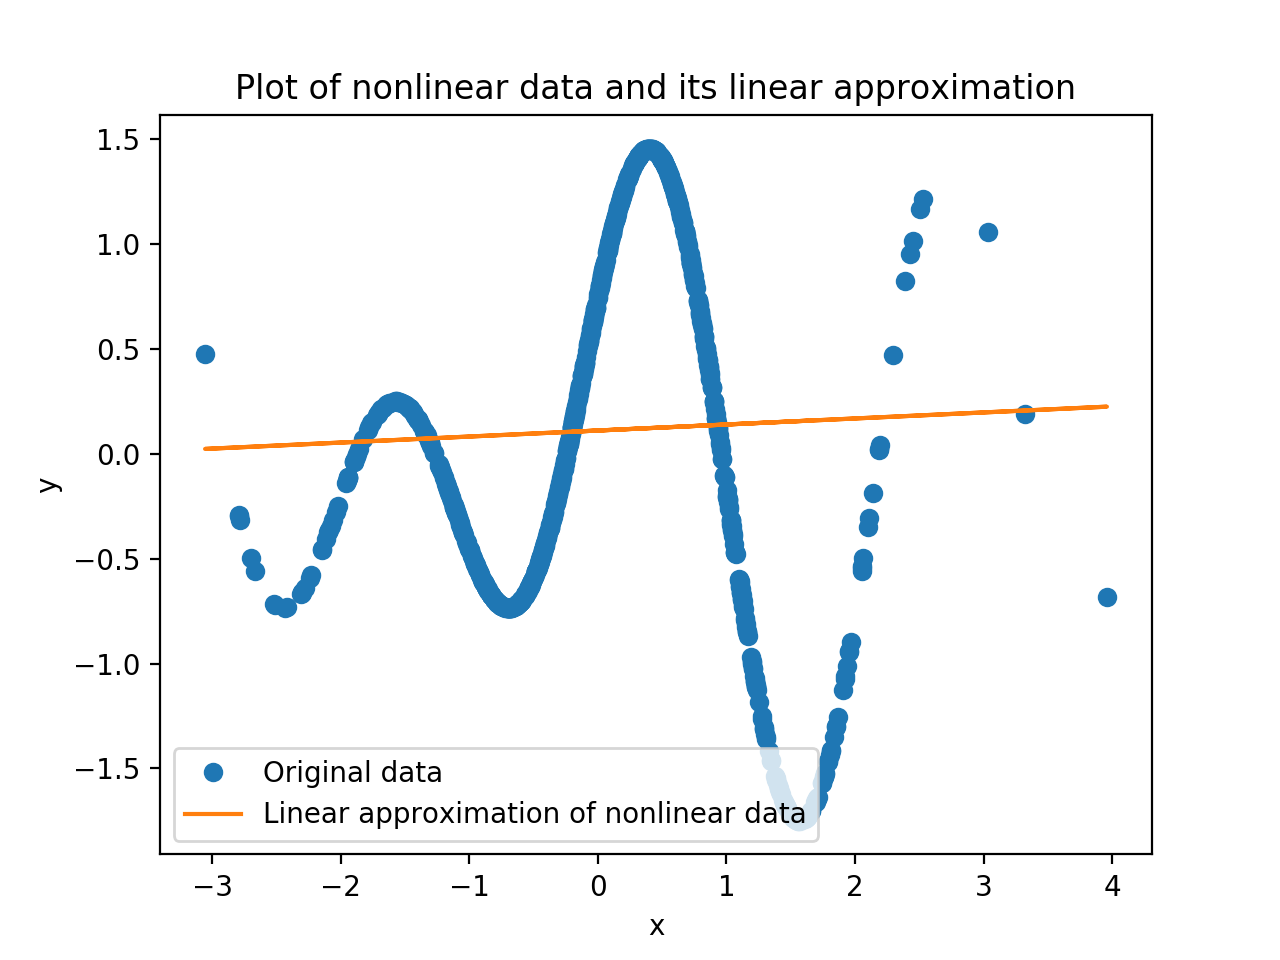
\includegraphics[width=0.7\textwidth]{../plots/task1_part2.png}
\caption{Nonlinear data and its linear approximation}
\label{fig:task1_2}
\end{figure}
Part 3:
After we tried to approximate the nonlinear dataset with a linear function in part 2, we now try to approximate the unknown nonlinear function with a combination of radial basis function:
\begin{equation*}
	\phi_l(x) = \exp(-||x_l -x||^2/\epsilon^2)
\end{equation*}
$x_l$ is the center of the basis function and usually just a randon point of the data set. There is one $x_l$ for each radial basis function. We have to choose how many basis functions L  we use to approximate the nonlinear function. Besides, we have to choose $\epsilon$ appropriately.
We choose 
Figure \ref{fig:task1_3} shows the original data in blue and the approximated function which makes use of radial basis functionsn in orange. It can be easily seen that the approximation is by far better than the linear approximation of part 2. In general the approximation fits the original function quite well.
\begin{figure}[H]
\centering
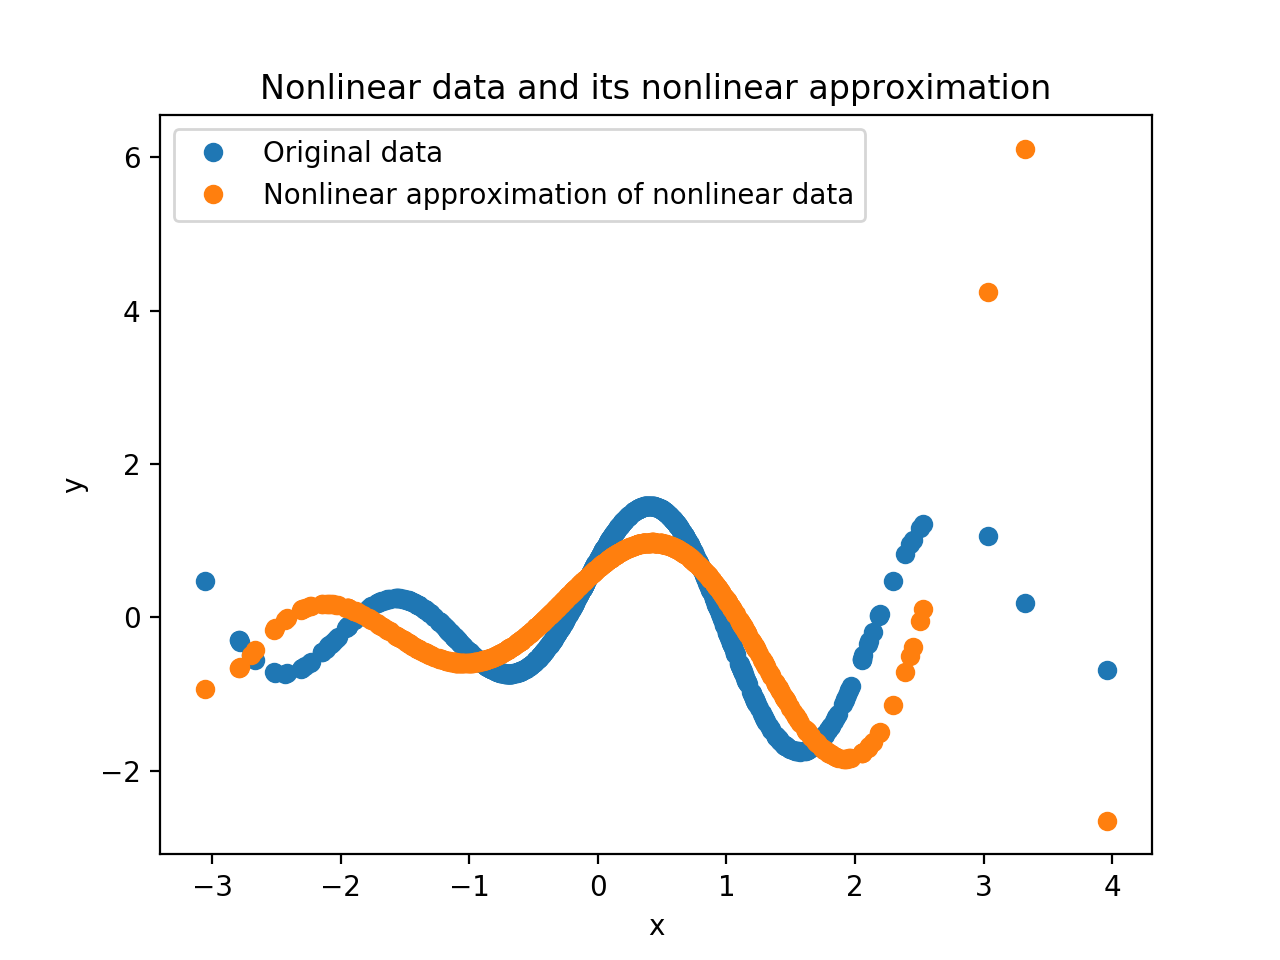
\includegraphics[width=0.7\textwidth]{../plots/task1_part3.png}
\caption{Nonlinear data and its nonlinear approximation with radial basis functions}
\label{fig:task1_3}
\end{figure}
\end{task}
\begin{task}{2, First step of a single pedestrian}
They stepped successfully (see figure).
\end{task}

\begin{task}{3, Approximating nonlinear vector fields}
- not done -
\end{task}
\begin{task}{4, Obstacle avoidance}
Pedestrians can avoid obstacles, using Dijkstras algorithm. See figure.
\end{task}
\begin{task}{5, Tests}
\begin{enumerate}
\item[TEST1:] RiMEA scenario 1 (straight line, ignore premovement time)\\
- not done, but citing RiMEA guidelines -
\item[TEST2:] RiMEA scenario 4 (fundamental diagram, be careful with periodic boundary conditions).\\
- test successful - 
\item[TEST3:] RiMEA scenario 6 (movement around a corner).\\
- test successful - 
\item[TEST4:] RiMEA scenario\\
- test successful - 
\end{enumerate}
\end{task}



\end{document}